\documentclass[a4paper, 12pt, titlepage]{article}

% osnovni paketi za jezik in kodiranje znakov
\usepackage[slovene]{babel} 
\usepackage[utf8]{inputenc}
\usepackage[T1]{fontenc}
\usepackage{lmodern}

% dodatni paketi
\usepackage{amsmath, amssymb, amsthm}
\usepackage[font=small, center]{caption}
\usepackage[hidelinks]{hyperref}
\usepackage{graphicx}
\usepackage{wrapfig}
\usepackage{float}     
\usepackage{geometry}
\geometry{tmargin=1.5in, textwidth=6.5in}
\usepackage[table]{xcolor} % http://ctan.org/pkg/xcolor
\usepackage{biblatex}
\addbibresource{literatura.bib}

% priprava strani
\pagestyle{headings}

\begin{document}

\begin{titlepage}
    \begin{center}
        \large
        Fakulteta za matematiko in fiziko\\
        \vspace{8cm}
        \Huge
        \textbf{Računanje določenega integrala s trikotniki} \\
        \vspace{7cm}
        \large
        Terezija Krečič\\
        Pedagoška matematika\\
        \vspace{1cm}
        Mentor: Uroš Kuzman\\
        \vspace{0.5cm}
        Ljubljana\\
        28. 5. 2023
    \end{center}
\end{titlepage}

\tableofcontents
\newpage

%%%%%%%%%%%%%%%%%%%%%%%%%%%%%%%%%%%%%%%%%%%%%%
\section{Uvod}

Naj bo $ f: [a,b] \rightarrow \mathbb{R} $ zvezna in pozitivna funkcija. Ploščino pod njenim grafom tipično aproksimiramo z Riemannovo vsoto oz. pravokotniki, da v limiti dobimo vrednost $ \int_{a}^{b}f(x)dx $. V nalogi si bomo ogledali metodo, ki integral konveksnih funkcij izračuna s pomočjo trikotnih območij.

Naš pristop bo temeljil na generiranju goste\footnote{Množica D je \emph{gosta} v topološkem prostoru $ X $ natanko tedaj, kadar je presek množice $ D $ z vsako neprazno odprto podmnožico v $ X $ neprazen. V našem primeru to pomeni, da se v vsakem odprtem podintervalu intervala integriranja nahaja vsaj en element iz te množice $ D $.} podmnožice intervala, po katerem integriramo, pri čemer si bomo za lažjo predstavitev te podmnožice pomogali z neskončnim binarnim drevesom. V postopku bomo s funkcijo, ki jo integriramo, ter izbiro delilnih točk intervala (tj. vozlišč drevesa) generirali vrsto, ki bo ponazarjala ploščino trikotnih območij pod funkcijo. Videli bomo, da lahko dobimo znano ali manj znano vrsto, naš cilj pa je določiti, ali divergira ali konvergira in če, h kateri vrednosti. Izkazalo se bo, da to ne bo vedno enostavno.


\newpage
%%%%%%%%%%%%%%%%%%%%%%%%%%%%%%%%%%%%%%%%%%%%%%
\section{Motivacijski primer}

Za boljšo predstavo o ideji integracije preko trikotnikov si poglejmo konkreten primer funkcije $ f(x) = \frac{1}{x} $ na intervalu $ (0, \infty) $. Gosto podmnožico definicijskega območja $ (0, \infty) $ generirajmo na sledeč način:

Začnimo z mejama intervala $ 0 $ in $ \infty $. Med njiju vrinimo delilno točko $ 1 $, s čimer dobimo podintervala $ (0, 1] $ in $ [1, \infty) $. Vsakega izmed njiju razdelimo z dodatnima delilnima točkama $ 1/2 $ in $ 2 $. Dobimo štiri podintervale osnovnega intervala, in zopet vsakega razdelimo tako, da končne intervale razpolovimo, v skrajnem desnem (neskončnem) intervalu pa za delilno točko izberemo naslednjo potenco števila $ 2 $ (torej v tem primeru $ 4 $). S tem postopkom nadaljujemo in tako dobimo neskončno binarno drevo, kot je prikazano na sliki~\ref{uvodni_primer_drevo}.

\begin{figure}[h]
    \centering
    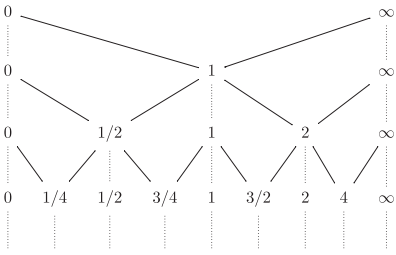
\includegraphics[width=0.45\textwidth]{slike/uvodni_primer_drevo.png}
    \caption{Vzeto iz~\cite{osnovni_clanek}.}
    \label{uvodni_primer_drevo}
\end{figure}

Opazimo (in tudi vemo), da sta $ x $- in $ y $-osi asimptoti na graf $ f $, torej nekakšni tangenti na $ f $ v točkah $ 0 $ in $ \infty $ (slednja seveda ni točka). Generiramo novo tangento na graf $ f $ v prvi točki drevesa, ki leži med $ 0 $ in $ \infty $. Te tri tangente se sekajo in skupaj tvorijo trikotnik, ki leži pod grafom $ f $, in pokriva del območja prvega kvadranta. Postopek ponovimo, le da sedaj trikotnike tvorimo v do sedaj s trikorniki še nepokritem območju -- vzamemo tangente v naslednjih točkah v drevesu: $ 1/2 $ in $ 2 $. Dobimo trikotnike, kot kaže slika~\ref{uvodni_primer_prvi_trikotniki}. V naslednjem koraku bi vzeli tangente v naslednjih štirih točkah: $ 1/4 $, $ 3/4 $, $ 3/2 $ in $ 4 $. S ponavljanjem postopka v limiti trikotniki pokrijejo celotno območje pod grafom funkcije $ f $.

\begin{figure}[h]
    \centering
    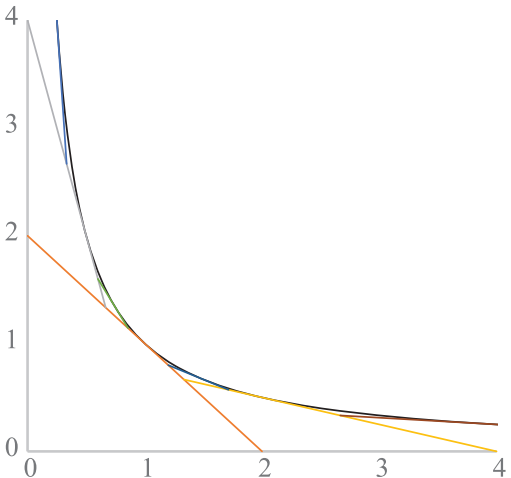
\includegraphics[width=0.3\textwidth]{slike/uvodni_primer_prvi_trikotniki.png}
    \caption{Prve tri tangente v particiji območja na trikotnike. Vzeto iz~\cite{osnovni_clanek}.}
    \label{uvodni_primer_prvi_trikotniki}
\end{figure}

Preprost izračun pokaže, da je ploščina vsakega trikotnika, ki z eno stranico leži na eni od koordinatnih osi (razen prvega trikotnika z ogliščem v izhodišču) konstantna z vrednostjo $ 2/3 $ (gl. sliko~\ref{ploscina_trikotnika_2^n}).

\begin{figure}[h]
    \centering
    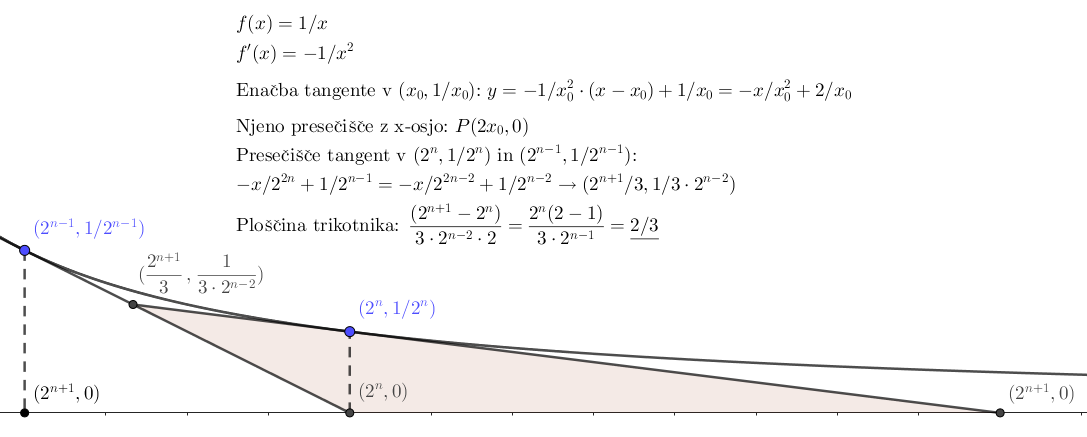
\includegraphics[width=\textwidth]{slike/ploscina_trikotnika_2^n.png}
    \caption{Izračun ploščine trikotnika ob osi.}
    \label{ploscina_trikotnika_2^n}
\end{figure}

Iz tega sledi, da je ploščina pod območjem (ki je vsota ploščin vseh trikotnikov) navzgor neomejena, saj je divergentna že vsota ploščin trikotnikov ob oseh. To je v skladu z vrednostjo izlimitiranega integrala $ \int_{0}^{\infty}\frac{1}{x}dx $.

Tako smo na primeru pokazali idejo -- z razdelitvijo območja na trikotnike lahko povežemo ploščino pod grafom in vsoto neskončne vrste (ki ustreza ploščini teh trikotnikov). V limiti, ko povečujemo število delilnih točk, dobimo ravno ploščino pod grafom.

Sedaj lahko raziščemo obnašanje teh vrst na primerih različnih funkcij in na različnih števnih gostih podmnožic.


%%%%%%%%%%%%%%%%%%%%%%%%%%%%%%%%%%%%%%%%%%%%%%
\section{Splošnejša obravnava problema}

Pri Riemannovem integralu poskrbimo za vedno finejšo particijo intervalov, iz katere so ustvarjena pravokotna območja. Le-ta skupaj v limiti, ko gre širina podintervalov proti 0, tvorijo območje pod grafom. Naš pristop je podoben, le da mora biti zaporedje particij dovolj organizirano, da lahko dobimo ustrezne trikotnike. En način lepšega pregleda točk pa nam omogoča neskončno binarno drevo.

Z določanjem zaporedja particij iz drevesa naš proces generiranja trikotnikov, ki napolnijo območje pod grafom funkcije $ f $, potrebuje le nekaj ključnih predpostavk:

\begin{enumerate}
    \item \label{predpostavka_1} Funkcija $ f $ je definirana na intervalu oblike $(0, \infty)$, $[0,\infty)$, $(0,a]$ ali $[0,a]$, kjer je $ 0 < a < \infty $, in sta $x$- in $y$-os v točkah 0 ter $a$ (oz. v $ \infty $) njeni tangenti (oz. asimptoti, odvisno od oblike intervala).
    \item \label{predpostavka_2} Funkcija $ f $ je dvakrat zvezno odvedljiva, strogo monotono padajoča ($ f'(x) < 0 $) in strogo konveksna ($ f''(x) > 0 $) za vsak $ x \in A$ (razen v krajiščih), kjer je $ A $ interval oblike, kot ga navaja točka~\ref{predpostavka_1}.
    \item \label{predpostavka_3} Množica, generirana iz neskončnega binarnega drevesa, je gosta podmnožica intervala $ A $.
\end{enumerate}

Te tri predpostavke so dovolj. Predpostavka~\ref{predpostavka_1} zagotavlja, da bosta dve stranici prvega trikotnika ležali na koordinatnih oseh. Predpostavka~\ref{predpostavka_2} poskrbi, da se novo generirane tangente tako razlikujejo od tangent iz prejšnjega koraka, da se tretja stranica novega trikotnika ne prekriva s prejšnjimi, sam trikotnik pa leži pod grafom. Predpostavka~\ref{predpostavka_3} pomeni, da se bo vsaka točka $ (x_0, y_0) $ v prvem kvadrantu, ki leži pod grafom, nahajala v vsaj kakšnem trikotniku.

V resnici pa s tem precej omejimo izbiro primernih funkcij. Vendar se da vsako funkcijo razdeliti na območja, ki jim z ustrezno prilagoditvijo lahko priredimo naš postopek (npr. pri konkavno funkciji vzamemo območje \emph{nad} grafom).

Računanje ploščine kateregakoli od teh trikotnikov je idejno preprost izračun. Za primer vzemimo tri zaporedne točke iz nekega istega nivoja drevesa: $ 0 < x_1 < x_{1,2} < x_2 $. Naj bo točka $ x_{1,2} $ generirana iz prejšnjih zaporednih točk $ x_1 $ in $ x_2 $. Znamo izračunati tangente na graf $ f $ v teh treh točkah ter medsebojna presečišča, kar so ravno vsi trije vrhovi novega trikotnika, iz koordinat oglišč pa znamo izračunati ploščino trikotnika. V konkretnem primeru je računanje dokaj enostavno, v splošnem pa je ploščina tega trikotnika enaka 

\begin{equation}
    \label{splosna_ploscina_formula}
    P = \frac{A^2}{2B}\text{,}
\end{equation}

kjer sta

\begin{align*}
    A =  &f'(x_1)f'(x_{1,2})(x_1 - x_{1,2}) + f'(x_1)f'(x_2)(x_2 - x_1) \\
&+ f'(x_2)f'(x_{1,2})(x_{1,2} - x_2) + f(x_1)(f'(x_2) - f'(x_{1,2})) \\
&+ f(x_2)(f'(x_{1,2}) - f'(x_1)) + f(x_{1,2})(f'(x_1) - f'(x_2))
\end{align*}

in
$$
B = (f'(x_1) - f'(x_{1,2}))(f'(x_1) - f'(x_2))(f'(x_2) - f'(x_{1,2}))\text{.}
$$

(To lahko izračunamo z računalnikom, za primer izračuna gl. sliko~\ref{splosna_ploscina}.)

\begin{figure}[h!]
    \centering
    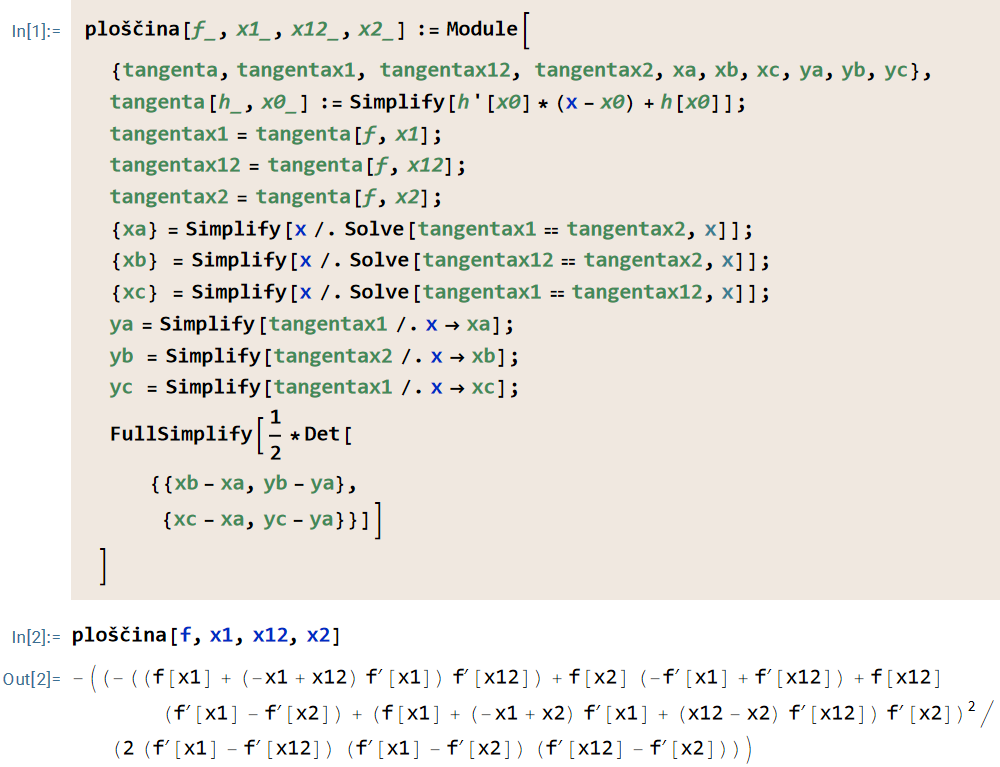
\includegraphics[width=0.8\textwidth]{slike/splosna_ploscina.png}
    \caption{Primer funkcije v programu Wolfram Mathemtatica, ki izračuna splošno ploščino (pod predpostavko, da se vse tri tangente paroma sekajo).}
    \label{splosna_ploscina}
\end{figure}


%%%%%%%%%%%%%%%%%%%%%%%%%%%%%%%%%%%%%%%%%%%%%%
\section{Ilustrativen primer} \label{ilustrativen_primer}

Vzemimo funkcijo $ g(x) = (1 - \sqrt{x})^2 $ na $ [0, 1] $ in drevo, ki ga prikazuje slika~\ref{ilustrativen_primer_drevo}. Vsako novo vozlišče se nahaja natanko med prejšnjima dvema (če odmislimo kvadriranje).

\begin{figure}[h!]
    \centering
    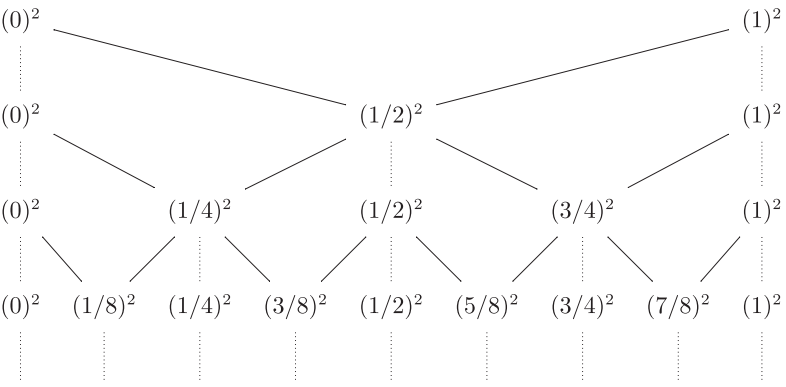
\includegraphics[width=0.7\textwidth]{slike/ilustrativen_primer_drevo.png}
    \caption{Vzeto iz~\cite{osnovni_clanek}.}
    \label{ilustrativen_primer_drevo}
\end{figure}

Zlahka preverimo, da za $ g $ in to drevo veljajo vse tri potrebne predpostavke. Radi bi izračunali ploščino pod grafom funckije $ g $ preko trikotnikov (z Riemannovim integralom enostavno dobimo rezultat 1/6).

Označimo nivoje drevesa z $ n $. Nivo $ 0 $ sta točki $ (0)^2 $ in $ (1)^2 $, nivo $ 1 $ točke $ (0)^2 $, $ \bigl(\frac{1}{2}\bigr)^2 $ in $ (1)^2 $, nivo $ 2 $ točke $ (0)^2 $, $ \bigl(\frac{1}{4}\bigr)^2 $, $ \bigl(\frac{1}{2}\bigr)^2 $, $ \bigl(\frac{3}{4}\bigr)^2 $, in $ (1)^2 $ itd. V splošnem torej nivo $ n $ predstavljajo točke $ (0)^2 $, $ \bigl(\frac{1}{2^n}\bigr)^2 $, $ \bigl(\frac{2}{2^n}\bigr)^2 $, $ \bigl(\frac{3}{2^n}\bigr)^2 $, \ldots, $ \bigl(\frac{2^n-2}{2^n}\bigr)^2 $, $ \bigl(\frac{2^n-1}{2^n}\bigr)^2 $ in $ (1)^2 $. Z vsakim nivojem dobimo nove točke, s tem pa tudi nove trikotnike -- natančneje, v nivoju n generiramo $ 2^{n-1} $ novih točk/trikotnikov.

Izkaže se, da je ploščina trikotnikov, ki jih dobimo v vsakem nivoju, enaka in odvisna le od $ n $. Do nje pridemo postopoma: najprej premislimo, da je vsak nov trikotnik v nivoju $ n $ odvisen od treh sosednjih točk na tem nivoju, od katerih je srednja tista, ki je na novo generirana. Tako lahko nivo $ n $ razdelimo na $ 2^{n-1} $ trojic: $ \{(0)^2, \bigl(\frac{1}{2^n}\bigr)^2,\bigl(\frac{2}{2^n}\bigr)^2\} $, $ \{\bigl(\frac{2}{2^n}\bigr)^2, \bigl(\frac{3}{2^n}\bigr)^2, \bigl(\frac{4}{2^n}\bigr)^2\} $, \ldots, $ \{\bigl(\frac{2^n-2}{2^n}\bigr)^2, \bigl(\frac{2^n-1}{2^n}\bigr)^2, (1)^2\}$. Označimo s $ k $ zaporedno mesto novo generirane točke v $ n $-tem nivoju, torej $ k = 1, 3, 5, \ldots, 2^n-1 $. Za vsak $ k $ lahko s pomočjo formule~\ref{splosna_ploscina_formula} izračunamo ploščino novega trikotnika, ki ima za oglišča presečišča tangenta v točkah $ \{\bigl(\frac{k-1}{2^n}\bigr)^2, \bigl(\frac{k}{2^n}\bigr)^2, \bigl(\frac{k+1}{2^n}\bigr)^2\} $. Ploščina je res neodvisna od $ k $ in znaša $ \frac{1}{2^{3n}} $.

Sedaj lahko izračunamo ploščino pod grafom funkcije $ g $. Trikotnike dobimo od nivoja $ 1 $ naprej, zato je $ n = 1, 2, 3, 4, \ldots $. Na $ n $-tem koraku dobimo $ 2^{n-1} $ novih trikotnikov s ploščino $ \frac{1}{2^{3n}} $. Premisliti moramo le uvedbo nove spremenljivke, ki bo namesto $ k $ tekla po zaporednih celih številih: vzamemo npr. $ t = \frac{k-1}{2} $, torej $ t = 0, 1, 2, 3, \ldots, 2^{n-1}-1 $. Ploščina pod grafom je tako res enaka

\begin{equation*}
    \sum_{n=1}^{\infty} \sum_{t=0}^{2^{n-1}-1} \frac{1}{2^{3n}} = \sum_{n=1}^{\infty} \frac{2^{n-1}}{2^{3n}} = \sum_{n=1}^{\infty} \frac{1}{2^{2n+1}} = \sum_{n=0}^{\infty} \frac{1}{2^{2n+3}} = \frac{1}{2^3} \frac{1}{1-\frac{1}{2^2}} = \frac{1}{6}\text{.}
\end{equation*}

\begin{figure}[h!]
    \centering
    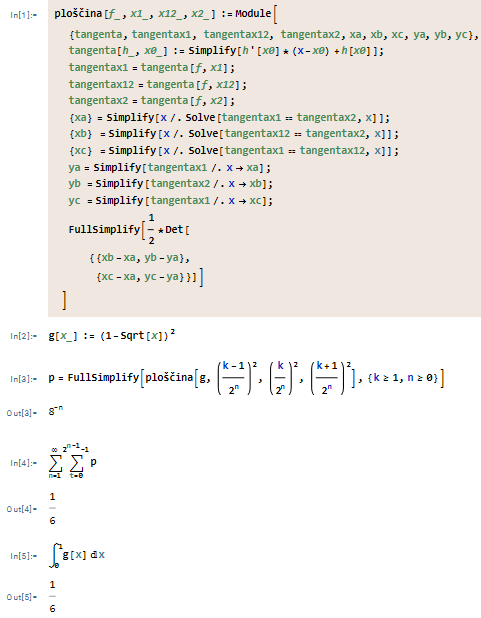
\includegraphics[width=0.8\textwidth]{slike/ilustrativen_primer_wolfram.png}
    \caption{Izračun ploščine trikotnikov iz $ n $-tega nivoja danega drevesa ter celotna ploščina pod območjem funkcije $ g $.}
    \label{ilustrativen_primer_wolfram}
\end{figure}

Ta primer med drugim tudi prikazuje še en način generiranja gostih podmnožic domene funkcije.

%%%%%%%%%%%%%%%%%%%%%%%%%%%%%%%%%%%%%%%%%%%%%%
\section[Generiranje gostih podmnožic z uporabo Stern-Brocotovega drevesa]{Generiranje gostih podmnožic z uporabo\\ Stern-Brocotovega drevesa \sectionmark{Stern-Brocotovo drevo}}
\sectionmark{Stern-Brocotovo drevo}

Še en način razdelitve intervala $ [0, \infty) $ na sliki~\ref{stern-brocot_tree} prikazuje t.i. Stern-Brocotovo drevo\footnote{angl. Stern-Brocot tree, op. prev.}. Neodvisno drug od drugega sta ga odkrila nemški matematik Moritz Stern l. 1858 in francoski urar Achille Brocot l. 1861. Drevo se začne z mejama intervala, ki ju lahko zapišemo v obliki $ \frac{0}{1}$ in $ \frac{1}{0} $, števila v drevesu pa generiramo kot mediante sosednjih ulomkov na istem nivoju (\emph{mediant} dveh racionalnih števil $ \frac{a}{b} $ in $ \frac{c}{d} $ je definiran kot $ \frac{a+c}{b+d} $).

\begin{figure}[h!]
    \centering
    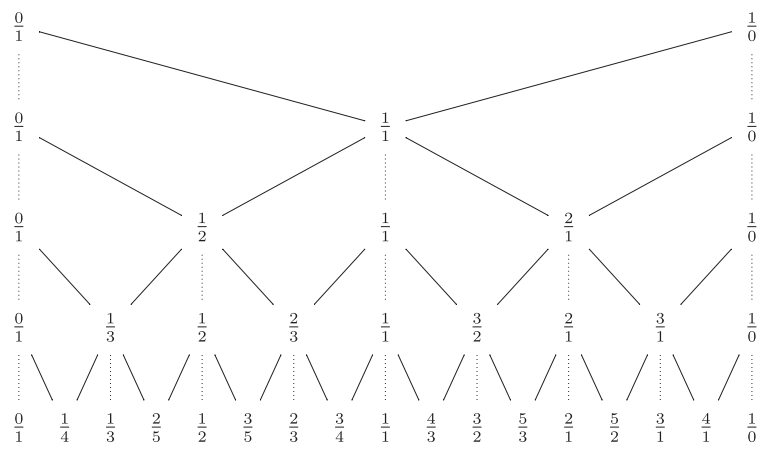
\includegraphics[width=0.8\textwidth]{slike/stern-brocot_tree.png}
    \caption{Stern-Brocotovo drevo. Vzeto iz~\cite{osnovni_clanek}.}
    \label{stern-brocot_tree}
\end{figure}

\subsection{Lastnosti Stern-Brocotovega drevesa}

\begin{enumerate}
    \item \label{prva_znacilnost}
    Za sosednja ulomka istega nivoja drevesa $ \frac{a}{b} < \frac{c}{d} $ velja $ \frac{a}{b} < \frac{a+c}{b+d} < \frac{c}{d} $. Preprost računski dokaz prepuščam bralcu.
    \item Za sosednja ulomka $ \frac{a}{b} < \frac{c}{d} $ je očitno $ bc - ad > 0 $. Velja celo več: $ bc - ad = 1 $.
    
    To dokažemo z indukcijo na nivojih drevesa. Za 0-ti in prvi nivo trditev očitno velja. Recimo sedaj, da velja tudi za vse do $ n $-tega nivoja. V $ n+1$-vem nivoju skonstruiramo novo število, za katerega iz~\ref{prva_znacilnost} velja $ \frac{a}{b} < \frac{a+c}{b+d} < \frac{c}{d} $. Upoštevamo indukcijsko predpostavko in izračunamo: $ c(b+d) - d(a+c) = bc-ad = 1 $ ter $ b(a+c) - a(b+d)  = bc-ad = 1 $.
    \item Vsak element drevesa je pozitiven okrajšan ulomek ter vsaka sosednja imenovalca v isti vrsti sta si tuja (oboje dokažemo z indukcijo in protislovjem) in ni težko premisliti, da se v Stern-Brocotovem drevesu pojavijo prav vsa pozitivna racionalna števila.
\end{enumerate}

\subsection{Ploščina pod grafom funkcije $ g $}

Izračunajmo ploščino pod grafom iste funkcije $ g(x) = (1 - \sqrt{x})^2 $, ki smo jo definirali v poglavju~\ref{ilustrativen_primer}, le da so delilne točke intervala $ [0,1] $ sedaj kvadratne vrednosti vozlišč leve polovice Stern-Brocotovega drevesa. V funkcijo~\ref{splosna_ploscina_formula} za splošno ploščino damo splošne tri zaporedne točke $ \frac{a}{b} < \frac{a+c}{b+d} < \frac{c}{d} $, ki na enem koraku generirajo nov trikotnik, in dobimo $ \frac{1}{2b^2d^2(b+d)^2} $. Vrsta za izračun ploščine se po razmisleku, da v celotni levi polovici drevesa $ b $ in $ d $ pretečeta vsa naravna števila (ker pa imata vsaka sosednja ulomka tuje imenovalce, vzamemo le tuje pare $ (b,d) $) torej glasi in je po izračunu v prejšnjem poglavju enaka:

\begin{equation}
    \sum_{\substack{b,d=1 \\ (b,d)=1}}^{\infty} \frac{1}{2b^2d^2(b+d)^2} = \frac{1}{6}\text{.}
    \label{SB_ilustrativen_primer}
\end{equation}

S tem primerom smo pokazali, kako različna delitev istega intervala porodi drugačno obliko neskončne vrste. Kot zanimivost -- formula~\ref{SB_ilustrativen_primer} je posebni primer bolj splošne funkcije, imenovane \emph{Mordell-Tornheim zeta funkcija}, ki ima splošno obliko

\begin{equation}
    \sum_{(m,n)=1}^{\infty} \frac{1}{m^{s_1}n^{s_2}(m+n)^{s3}}\text{.}
\end{equation}


%%%%%%%%%%%%%%%%%%%%%%%%%%%%%%%%%%%%%%%%%%%%%%
\section{Razred konvergentnih vrst}

Izkaže se, da če za funkcijo iz motivacijskega primera, $ f(x) = \frac{1}{x} $, uporabimo zgornji dve drevesi, dobimo novi različni divergentni vrsti. Ali znamo generirati konvergentno vrsto iz funkcij, podobnih $ g $ iz~\ref{ilustrativen_primer}? Na primer iz dela enotske krožnice $ (x-1)^2+(y-1)^2=1 $ na $ [0,1] \times [0,1]$ ali funkcije $ y = (1-\sqrt[3]{x})^3 $ na $ [0,1] $? Izkaže se, da preoblikovanje drevesa pripomore k poenostavljenemu računanju ploščin trikotnikov, vendar v obeh primerih ne dobimo neke enostavne, lepe vrste.

Primer funkcije, kjer pa lahko dobimo družino neskončnih vrst še kar lepe oblike, je $ f(x)=x^{-1/r} $ na $ [0,1] $ za $ r \in \mathbb{N}; r > 1 $. Vzemimo drevo, kot kaže slika~\ref{r_drevo} (za $ r = 2 $ dobimo drevo iz poglavja~\ref{ilustrativen_primer}):

\begin{figure}[h!]
    \centering
    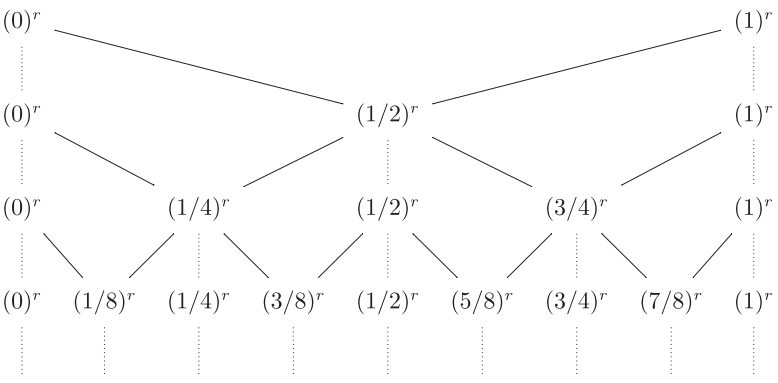
\includegraphics[width=0.8\textwidth]{slike/r_drevo.png}
    \caption{Vzeto iz~\cite{osnovni_clanek}.}
    \label{r_drevo}
\end{figure}

Na enak način Kot v poglavju~\ref{ilustrativen_primer} izračunamo ploščino trikotnika v $ n $-tem nivoju iz trojice zaporednih točk $ \{\bigl(\frac{k-1}{2^n}\bigr)^r, \bigl(\frac{k}{2^n}\bigr)^r, \bigl(\frac{k+1}{2^n}\bigr)^r\} $, kjer $ k = 1, 3, 5, \ldots, 2^n-1 $ označuje zaporedno mesto novo generirane točke v $ n $-tem nivoju. Ploščina je tokrat odvisna od $ k $ in znaša

\begin{equation*}
    P_k = \frac{
        \bigl(((k-1)k)^r + (k(k+1))^r - 2(k^2-1)^r\bigr)^2(1+r)^2
    }{
        2^{nr-n+1} r \bigl(k^{r+1} - (k-1)^{r+1}\bigr) \bigl((k+1)^{r+1} - (k-1)^{r+1}\bigr) \bigl((k+1)^{r+1} - k^{r+1}\bigr)
    }\text{.}
\end{equation*}

Za izračun celotne ploščine zopet uporabimo zvezo $ t = \frac{k-1}{2} $:

\begin{equation}
    P = \sum_{n=0}^{\infty} \sum_{t=0}^{2^n-1}
    \frac{
        \bigl(t^r (2t+1)^r - 2^{r+1} t^r (t+1)^r + (2t+1)^r(t+1)^r\bigr)^2(1+r)^2
    }{
        2^{nr-n+1}r
        \bigl((2t+1)^{r+1}-(2t)^{r+1}\bigr)
        \bigl((t + 1)^{r+1} - t^{r+1}\bigr)
        \bigl((2t + 2)^{r+1} - (2t+1)^{r+1}\bigr)
    }\text{,}
    \label{splosen_r}
\end{equation}

\begin{equation}
    \text{ kjer za } r = 2 \text{ dobimo }
    P' = \sum_{n=0}^{\infty} \sum_{t=0}^{2^n-1} \frac{9(6t^2+6t+1)^2}{2^n(1+27(2t+1)^6)}\text{.}
    \label{r2_primer}
\end{equation}

Opazimo, da funkcija $ f $ ne ustreza povsem predpostavki~\ref{predpostavka_1}, saj na $ [0,1] $ $ x $-os ni njena tangenta (gl. sliko~\ref{r_funkcija}). Zato vrsta~\ref{splosen_r}, ki jo dobimo za splošen $ r $, ne konvergira k vrednosti $ \int_{0}^{1}f(x)dx $. Vendar je popravek k formuli enostaven -- izračunamo ploščino trapeznega območja, ki ni pokrito s trikotniki, ter to odštejemo od določenega integrala in dobimo vrednost vrste. Za $ r = 2 $ tako vrsta~\ref{r2_primer} konvergira k $ \int_{0}^{1}\frac{1}{x^{1/2}}dx - \frac{5}{4} = \frac{3}{4} $, za splošno funckijo $ f(x)=x^{-1/r} $ pa njena vrsta~\ref{splosen_r} konvergira proti

\begin{equation*}
    \int_{0}^{1}x^{-\frac{1}{2}}dx - \frac{2r+1}{2r} = \frac{r+1}{2r(r-1)}\text{.}
\end{equation*}

\begin{figure}[h!]
    \centering
    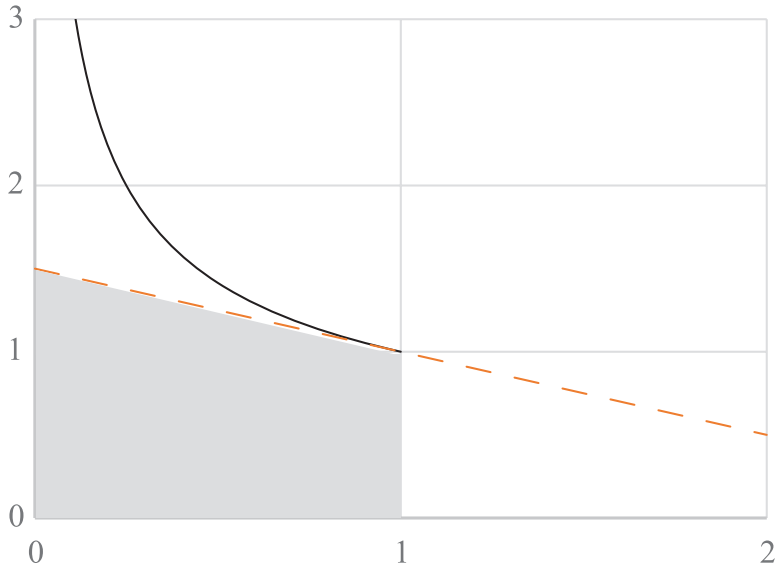
\includegraphics[width=0.5\textwidth]{slike/r_funkcija.png}
    \caption{Sivoobarvano območje pod $ f(x) = x^{-1/r} $ ni trikotnik. Vzeto iz~\cite{osnovni_clanek}.}
    \label{r_funkcija}
\end{figure}



%%%%%%%%%%%%%%%%%%%%%%%%%%%%%%%%%%%%%%%%%%%%%%
\section{Zaključek}

Glavna ideja računanja ploščine območja pod grafom s trikotniki je torej uporabiti neskončno binarno drevo, ki določen interval razdeli na goste podmnožice. Iz tega drevesa dobimo neskončno vrsto, ki je za isti določen integral pri različnih drevesih tudi sama različne oblike, njena vsota pa se seveda ne spremeni.

Tu se poraja vprašanje, kako sploh generiramo ta drevesa. Videli smo primere, kjer smo dobili vrsto, ki je nismo znali preprosto izračunati, torej kakršnakoli gosta delitev verjetno ne bo zadostovala. Torej kako lahko zagotovimo, da z nekim drevesom dobimo vrsto, ki jo znamo izračunati brez pomoči kalkulatorja? Naslednje vprašanje pa je, ali lahko naredimo obratno in če da, pod katerimi pogoji -- torej da iz dane vrste sproduciramo funkcijo, ki ji odgovarja?

Vsekakor so to vprašanja, ki zahtevajo veliko več poglobitve in v tem članku tako z njimi tudi zaključujem. Ideja se mi zdi dobra, vendar lepih primerov zaenkrat nisem našla veliko. Najbolj zanimiv del mi je uporaba te tehnike za dokaz divergence $ \int_0^\infty \frac{1}{x} dx $, ki je za srednješolce lahko v veliko zadovoljstvo, saj ne presega njihovega znanja in je hkrati zanje tudi dovoljšen izziv.



\newpage
%%%%%%%%%%%%%%%%%%%%%%%%%%%%%%%%%%%%%%%%%%%%%%
\newpage
\nocite{*}      % navede tudi vire, ki jih ne citiras
\printbibliography
%%%%%%%%%%%%%%%%%%%%%%%%%%%%%%%%%%%%%%%%%%%%%%
\end{document}